sources of great range error: causing corrupted CAERs: trajectory and map figure,
purple and cyan regions


\begin{figure}
  \definecolor{c3}{RGB}{41 160 203}
\definecolor{c4}{RGB}{231 138 195}
\definecolor{c5}{RGB}{92 53 102}
\definecolor{c6}{RGB}{252 233 79}



% GNUPLOT: LaTeX picture with Postscript
\begingroup
  \makeatletter
  \providecommand\color[2][]{%
    \GenericError{(gnuplot) \space\space\space\@spaces}{%
      Package color not loaded in conjunction with
      terminal option `colourtext'%
    }{See the gnuplot documentation for explanation.%
    }{Either use 'blacktext' in gnuplot or load the package
      color.sty in LaTeX.}%
    \renewcommand\color[2][]{}%
  }%
  \providecommand\includegraphics[2][]{%
    \GenericError{(gnuplot) \space\space\space\@spaces}{%
      Package graphicx or graphics not loaded%
    }{See the gnuplot documentation for explanation.%
    }{The gnuplot epslatex terminal needs graphicx.sty or graphics.sty.}%
    \renewcommand\includegraphics[2][]{}%
  }%
  \providecommand\rotatebox[2]{#2}%
  \@ifundefined{ifGPcolor}{%
    \newif\ifGPcolor
    \GPcolorfalse
  }{}%
  \@ifundefined{ifGPblacktext}{%
    \newif\ifGPblacktext
    \GPblacktexttrue
  }{}%
  % define a \g@addto@macro without @ in the name:
  \let\gplgaddtomacro\g@addto@macro
  % define empty templates for all commands taking text:
  \gdef\gplfronttext{}%
  \gdef\gplfronttext{}%
  \makeatother
  \ifGPblacktext
    % no textcolor at all
    \def\colorrgb#1{}%
    \def\colorgray#1{}%
  \else
    % gray or color?
    \ifGPcolor
      \def\colorrgb#1{\color[rgb]{#1}}%
      \def\colorgray#1{\color[gray]{#1}}%
      \expandafter\def\csname LTw\endcsname{\color{white}}%
      \expandafter\def\csname LTb\endcsname{\color{black}}%
      \expandafter\def\csname LTa\endcsname{\color{black}}%
      \expandafter\def\csname LT0\endcsname{\color[rgb]{1,0,0}}%
      \expandafter\def\csname LT1\endcsname{\color[rgb]{0,1,0}}%
      \expandafter\def\csname LT2\endcsname{\color[rgb]{0,0,1}}%
      \expandafter\def\csname LT3\endcsname{\color[rgb]{1,0,1}}%
      \expandafter\def\csname LT4\endcsname{\color[rgb]{0,1,1}}%
      \expandafter\def\csname LT5\endcsname{\color[rgb]{1,1,0}}%
      \expandafter\def\csname LT6\endcsname{\color[rgb]{0,0,0}}%
      \expandafter\def\csname LT7\endcsname{\color[rgb]{1,0.3,0}}%
      \expandafter\def\csname LT8\endcsname{\color[rgb]{0.5,0.5,0.5}}%
    \else
      % gray
      \def\colorrgb#1{\color{black}}%
      \def\colorgray#1{\color[gray]{#1}}%
      \expandafter\def\csname LTw\endcsname{\color{white}}%
      \expandafter\def\csname LTb\endcsname{\color{black}}%
      \expandafter\def\csname LTa\endcsname{\color{black}}%
      \expandafter\def\csname LT0\endcsname{\color{black}}%
      \expandafter\def\csname LT1\endcsname{\color{black}}%
      \expandafter\def\csname LT2\endcsname{\color{black}}%
      \expandafter\def\csname LT3\endcsname{\color{black}}%
      \expandafter\def\csname LT4\endcsname{\color{black}}%
      \expandafter\def\csname LT5\endcsname{\color{black}}%
      \expandafter\def\csname LT6\endcsname{\color{black}}%
      \expandafter\def\csname LT7\endcsname{\color{black}}%
      \expandafter\def\csname LT8\endcsname{\color{black}}%
    \fi
  \fi
    \setlength{\unitlength}{0.0500bp}%
    \ifx\gptboxheight\undefined%
      \newlength{\gptboxheight}%
      \newlength{\gptboxwidth}%
      \newsavebox{\gptboxtext}%
    \fi%
    \setlength{\fboxrule}{0.5pt}%
    \setlength{\fboxsep}{1pt}%
\begin{picture}(5000.00,1600.00)%
    \gplgaddtomacro\gplfronttext{%
      \colorrgb{0.15,0.15,0.15}%
      \put(468,160){\makebox(0,0)[r]{\strut{}\scriptsize $10^{-1}$}}%
      \colorrgb{0.15,0.15,0.15}%
      \put(368,586){\makebox(0,0)[r]{\strut{}\scriptsize $10^{0}$}}%
      \colorrgb{0.15,0.15,0.15}%
      \put(468,1013){\makebox(0,0)[r]{\strut{}\scriptsize $10^{+1}$}}%
      \colorrgb{0.15,0.15,0.15}%
      \put(468,1439){\makebox(0,0)[r]{\strut{}\scriptsize $10^{+2}$}}%
      \colorrgb{0.15,0.15,0.15}%
      \put(500,-60){\makebox(0,0){\strut{}\scriptsize $10^0$}}%
      \colorrgb{0.15,0.15,0.15}%
      \put(959,-60){\makebox(0,0){\strut{}\scriptsize $10^{+1}$}}%
      \colorrgb{0.15,0.15,0.15}%
      \put(1419,-60){\makebox(0,0){\strut{}\scriptsize $10^{+2}$}}%
      \colorrgb{0.15,0.15,0.15}%
      \put(1878,-60){\makebox(0,0){\strut{}\scriptsize $10^{+3}$}}%
    }%
    \gplgaddtomacro\gplfronttext{%
      \colorrgb{0.15,0.15,0.15}%
      \put(1349,-390){\makebox(0,0){\strut{}\footnotesize Area [m$^2$]}}%
      \colorrgb{0.00,0.00,0.00}%
      \put(1349,1859){\makebox(0,0){\strut{}\footnotesize Execution time vs area}}%
      \put(1100,1600){\makebox(0,0){\strut{}{\color{c3}{\rule[0.6mm]{0.3cm}{0.5mm}}} \scriptsize FastVGICP}}
      \put(1900,1600){\makebox(0,0){\strut{}{\color{c4}{\rule[0.6mm]{0.3cm}{0.5mm}}} \scriptsize \texttt{x1}}}
      \put(3500,1600){\makebox(0,0){\strut{}{\color{c5}{\rule[0.6mm]{0.3cm}{0.5mm}}} \scriptsize t minus \texttt{sm2}}}
      \put(4600,1600){\makebox(0,0){\strut{}{\color{c6}{\rule[0.6mm]{0.3cm}{0.5mm}}} \scriptsize Intersections}}
    }%
    \gplgaddtomacro\gplfronttext{%
      \colorrgb{0.15,0.15,0.15}%
      \put(2993,160){\makebox(0,0)[r]{\strut{}\scriptsize $0.0$}}%
      \colorrgb{0.15,0.15,0.15}%
      \put(2993,416){\makebox(0,0)[r]{\strut{}\scriptsize $0.2$}}%
      \colorrgb{0.15,0.15,0.15}%
      \put(2993,672){\makebox(0,0)[r]{\strut{}\scriptsize $0.4$}}%
      \colorrgb{0.15,0.15,0.15}%
      \put(2993,927){\makebox(0,0)[r]{\strut{}\scriptsize $0.6$}}%
      \colorrgb{0.15,0.15,0.15}%
      \put(2993,1183){\makebox(0,0)[r]{\strut{}\scriptsize $0.8$}}%
      \colorrgb{0.15,0.15,0.15}%
      \put(2993,1439){\makebox(0,0)[r]{\strut{}\scriptsize $1.0$}}%
      \colorrgb{0.15,0.15,0.15}%
      \put(3025,-60){\makebox(0,0){\strut{}\scriptsize $10^0$}}%
      \colorrgb{0.15,0.15,0.15}%
      \put(3506,-60){\makebox(0,0){\strut{}\scriptsize $10^{+1}$}}%
      \colorrgb{0.15,0.15,0.15}%
      \put(3987,-60){\makebox(0,0){\strut{}\scriptsize $10^{+2}$}}%
      \colorrgb{0.15,0.15,0.15}%
      \put(4468,-60){\makebox(0,0){\strut{}\scriptsize $10^{+3}$}}%
      \colorrgb{0.15,0.15,0.15}%
      \put(4949,-60){\makebox(0,0){\strut{}\scriptsize $10^{+4}$}}%
    }%
    \gplgaddtomacro\gplfronttext{%
      \colorrgb{0.15,0.15,0.15}%
      \put(3987,-390){\makebox(0,0){\strut{}\footnotesize Area [m$^2$]}}%
      \colorrgb{0.00,0.00,0.00}%
      \put(3987,1859){\makebox(0,0){\strut{}\footnotesize Timing breakdown vs area}}%
    }%
    \put(0,0){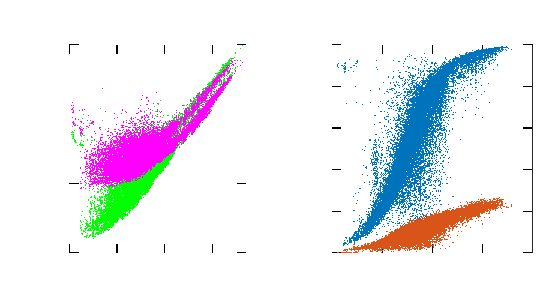
\includegraphics{./figures/experiments/c/time_analysis}}%
    \gplfronttext
  \end{picture}%
\endgroup

  \vspace{0.2cm}
  \caption{\small Left: CBGL's execution time with respect to environment area
           for two choices of overlying scan--to--map-scan matching
           (\texttt{sm2}) methods. In rough terms
           $time \text{ [sec]} = 17\cdot10^{-3}\cdot area \text{ [} \text{m}^2 \text{]}$.
           Right: Proportion of total execution time
           spent on (a) all operations up to and except for matching, and (b)
           computing map-scans, with respect to area}
  \label{fig:c:time_analysis}
\end{figure}


\begin{figure}%\hspace{0.5cm}
  % GNUPLOT: LaTeX picture with Postscript
\begingroup
  \makeatletter
  \providecommand\color[2][]{%
    \GenericError{(gnuplot) \space\space\space\@spaces}{%
      Package color not loaded in conjunction with
      terminal option `colourtext'%
    }{See the gnuplot documentation for explanation.%
    }{Either use 'blacktext' in gnuplot or load the package
      color.sty in LaTeX.}%
    \renewcommand\color[2][]{}%
  }%
  \providecommand\includegraphics[2][]{%
    \GenericError{(gnuplot) \space\space\space\@spaces}{%
      Package graphicx or graphics not loaded%
    }{See the gnuplot documentation for explanation.%
    }{The gnuplot epslatex terminal needs graphicx.sty or graphics.sty.}%
    \renewcommand\includegraphics[2][]{}%
  }%
  \providecommand\rotatebox[2]{#2}%
  \@ifundefined{ifGPcolor}{%
    \newif\ifGPcolor
    \GPcolorfalse
  }{}%
  \@ifundefined{ifGPblacktext}{%
    \newif\ifGPblacktext
    \GPblacktexttrue
  }{}%
  % define a \g@addto@macro without @ in the name:
  \let\gplgaddtomacro\g@addto@macro
  % define empty templates for all commands taking text:
  \gdef\gplfronttext{}%
  \gdef\gplfronttext{}%
  \makeatother
  \ifGPblacktext
    % no textcolor at all
    \def\colorrgb#1{}%
    \def\colorgray#1{}%
  \else
    % gray or color?
    \ifGPcolor
      \def\colorrgb#1{\color[rgb]{#1}}%
      \def\colorgray#1{\color[gray]{#1}}%
      \expandafter\def\csname LTw\endcsname{\color{white}}%
      \expandafter\def\csname LTb\endcsname{\color{black}}%
      \expandafter\def\csname LTa\endcsname{\color{black}}%
      \expandafter\def\csname LT0\endcsname{\color[rgb]{1,0,0}}%
      \expandafter\def\csname LT1\endcsname{\color[rgb]{0,1,0}}%
      \expandafter\def\csname LT2\endcsname{\color[rgb]{0,0,1}}%
      \expandafter\def\csname LT3\endcsname{\color[rgb]{1,0,1}}%
      \expandafter\def\csname LT4\endcsname{\color[rgb]{0,1,1}}%
      \expandafter\def\csname LT5\endcsname{\color[rgb]{1,1,0}}%
      \expandafter\def\csname LT6\endcsname{\color[rgb]{0,0,0}}%
      \expandafter\def\csname LT7\endcsname{\color[rgb]{1,0.3,0}}%
      \expandafter\def\csname LT8\endcsname{\color[rgb]{0.5,0.5,0.5}}%
    \else
      % gray
      \def\colorrgb#1{\color{black}}%
      \def\colorgray#1{\color[gray]{#1}}%
      \expandafter\def\csname LTw\endcsname{\color{white}}%
      \expandafter\def\csname LTb\endcsname{\color{black}}%
      \expandafter\def\csname LTa\endcsname{\color{black}}%
      \expandafter\def\csname LT0\endcsname{\color{black}}%
      \expandafter\def\csname LT1\endcsname{\color{black}}%
      \expandafter\def\csname LT2\endcsname{\color{black}}%
      \expandafter\def\csname LT3\endcsname{\color{black}}%
      \expandafter\def\csname LT4\endcsname{\color{black}}%
      \expandafter\def\csname LT5\endcsname{\color{black}}%
      \expandafter\def\csname LT6\endcsname{\color{black}}%
      \expandafter\def\csname LT7\endcsname{\color{black}}%
      \expandafter\def\csname LT8\endcsname{\color{black}}%
    \fi
  \fi
    \setlength{\unitlength}{0.0500bp}%
    \ifx\gptboxheight\undefined%
      \newlength{\gptboxheight}%
      \newlength{\gptboxwidth}%
      \newsavebox{\gptboxtext}%
    \fi%
    \setlength{\fboxrule}{0.5pt}%
    \setlength{\fboxsep}{1pt}%
\begin{picture}(4600.00,3000.00)%
    \gplgaddtomacro\gplfronttext{%
      \colorrgb{0.15,0.15,0.15}%
      \put(328,478){\makebox(0,0)[r]{\strut{}\small $c_0$}}%
      \colorrgb{0.15,0.15,0.15}%
      \put(328,1533){\makebox(0,0)[r]{\strut{}\small $500$}}%
      \colorrgb{0.15,0.15,0.15}%
      \put(328,2053){\makebox(0,0)[r]{\strut{}\small $1000$}}%
      \colorrgb{0.15,0.15,0.15}%
      \put(328,2573){\makebox(0,0)[r]{\strut{}\small $2000$}}%
      \colorrgb{0.15,0.15,0.15}%
      \put(460,80){\makebox(0,0){\strut{}\small $0.05$}}%
      \colorrgb{0.15,0.15,0.15}%
      \put(854,80){\makebox(0,0){\strut{}\small $5.0$}}%
      \colorrgb{0.15,0.15,0.15}%
      \put(1251,80){\makebox(0,0){\strut{}\small $10.0$}}%
      \colorrgb{0.15,0.15,0.15}%
      \put(1635,80){\makebox(0,0){\strut{}\small $\delta_0$}}%
      \colorrgb{0.15,0.15,0.15}%
      \put(2046,80){\makebox(0,0){\strut{}\small $20.0$}}%
    }%
    \gplgaddtomacro\gplfronttext{%
      \colorrgb{0.15,0.15,0.15}%
      \put(-160,1499){\rotatebox{90}{\makebox(0,0){\strut{}\small CAER [m]}}}%
      \colorrgb{0.15,0.15,0.15}%
      %\put(1253,-250){\makebox(0,0){\strut{}\small estimate error \footnotesize [(m$^2$ + rad$^2$)$^{1/2}$]}}%
    }%
    \gplgaddtomacro\gplfronttext{%
      \colorrgb{0.15,0.15,0.15}%
      \put(2835,300){\makebox(0,0)[r]{\strut{}\small $10^0$}}%
      \colorrgb{0.15,0.15,0.15}%
      \put(2835,700){\makebox(0,0)[r]{\strut{}\small $10^1$}}%
      \colorrgb{0.15,0.15,0.15}%
      \put(2835,1099){\makebox(0,0)[r]{\strut{}\small $10^2$}}%
      \colorrgb{0.15,0.15,0.15}%
      \put(2835,1499){\makebox(0,0)[r]{\strut{}\small $10^3$}}%
      \colorrgb{0.15,0.15,0.15}%
      \put(2835,1898){\makebox(0,0)[r]{\strut{}\small $10^4$}}%
      \colorrgb{0.15,0.15,0.15}%
      \put(2835,2298){\makebox(0,0)[r]{\strut{}\small $10^5$}}%
      \colorrgb{0.15,0.15,0.15}%
      \put(2835,2698){\makebox(0,0)[r]{\strut{}\small $10^5$}}%
      \colorrgb{0.15,0.15,0.15}%
      \put(2967,80){\makebox(0,0){\strut{}\small $0.05$}}%
      \colorrgb{0.15,0.15,0.15}%
      \put(3361,80){\makebox(0,0){\strut{}\small $5.0$}}%
      \colorrgb{0.15,0.15,0.15}%
      \put(3758,80){\makebox(0,0){\strut{}\small $10.0$}}%
      \colorrgb{0.15,0.15,0.15}%
      \put(4142,80){\makebox(0,0){\strut{}\small $\delta_0$}}%
      \colorrgb{0.15,0.15,0.15}%
      \put(4553,80){\makebox(0,0){\strut{}\small $20.0$}}%
    }%
    \gplgaddtomacro\gplfronttext{%
      \colorrgb{0.15,0.15,0.15}%
      %\put(2400,1499){\rotatebox{90}{\makebox(0,0){\strut{}\small rank in ascending CAER hierarchy}}}%
      \put(2400,1499){\rotatebox{90}{\makebox(0,0){\strut{}\small hypothesis' rank in CAER hierarchy}}}%
      \colorrgb{0.15,0.15,0.15}%
      \put(2300,-250){\makebox(0,0){\strut{}\small estimate error \footnotesize [(m$^2$ + rad$^2$)$^{1/2}$]}}%
    }%
    \put(0,0){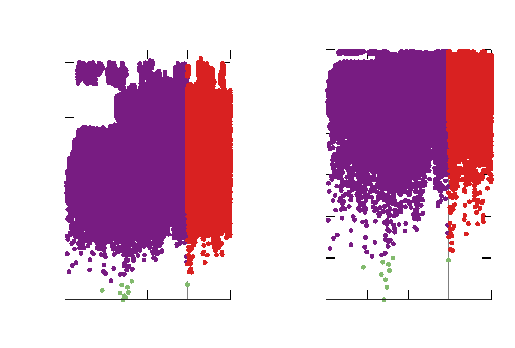
\includegraphics{./figures/h_not_fig}}%
    \gplfronttext
  \end{picture}%
\endgroup

  \vspace{0.7cm}
  \caption{\small Contrary to fig. \ref{fig:h_fig1}: the $\psi$-field (left)
           and \texttt{r}-field (right) of a configuration where Observation
           \ref{obs:observation_o} cannot be made: set $\mathcal{V}$ is
           empty of admissible pose estimates for $\delta < 4.5 \ (\text{m}^2 + \text{rad}^2)^{1/2}$.
           The effect is in fact produced due to the repetition of the
           immediate environment of the sensor more than once in the given map
           and its apparent dissimilarity to its corresponding portion of the
           map}
  \label{fig:h_not_fig1}
\end{figure}
